\chapter{Implementación}
En el siguiente capítulo se describe la implementación del sistema desarrollado durante la memoria. Se implementaron dos posibles arquitecturas para un sistema de reconocimiento de videos. La primera alternativa graba videos con el dispositivo móvil y los envía completos al servidor, para que este calcule sus descriptores y realice la búsqueda, llamamos a esta la alternativa \emph{centralizada} pues todos los cálculos son realizados en el servidor. La segunda alternativa del sistema realiza los cálculos de descriptores en el mismo dispositivo móvil que graba el video, luego solo es necesario enviar los descriptores calculados al servidor que ejecuta la búsqueda, llamamos a esta alternativa \emph{distribuida} pues los cálculos están repartidos entre el cliente y el servidor.

En ambas versiones del sistema el cliente corresponde a una aplicación Android implementada en el lenguaje de programación Java, mientras que el servidor fue implementado en Python usando Flask\footnote{\url{http://flask.pocoo.org/}}, un framework minimal para programación de servicios web. Se decidió este ambiente de programación para el servidor dada la familiaridad del alumno memorista con el framework y porque la implementación del servidor no requiere funcionalidad compleja que justifique usar herramientas más completas.

El capítulo se divide en una sección para la alternativa centralizada y otra para la distribuida. A su vez cada sección se divide en la implementación del cliente Android y el servidor.

\TODO{Pensar en mejores nombres para los sistemas alternativos}


\section{Sistema Centralizado}

La figura~\ref{arquitectura_centralizada} muestra la arquitectura de la versión centralizada del sistema. En esta versión el dispositivo móvil es usado solo para grabar un video corto. El archivo de video resultante es enviado al servidor (1), el cual calcula sus descriptores (2) y realiza la búsqueda en la base de datos (3), devolviendo los resultados al cliente (4).
A continuación se detalla la implementación de esta versión del sistema, separando el cliente Android del servidor.
	\begin{figure}[!h]
		\centering
		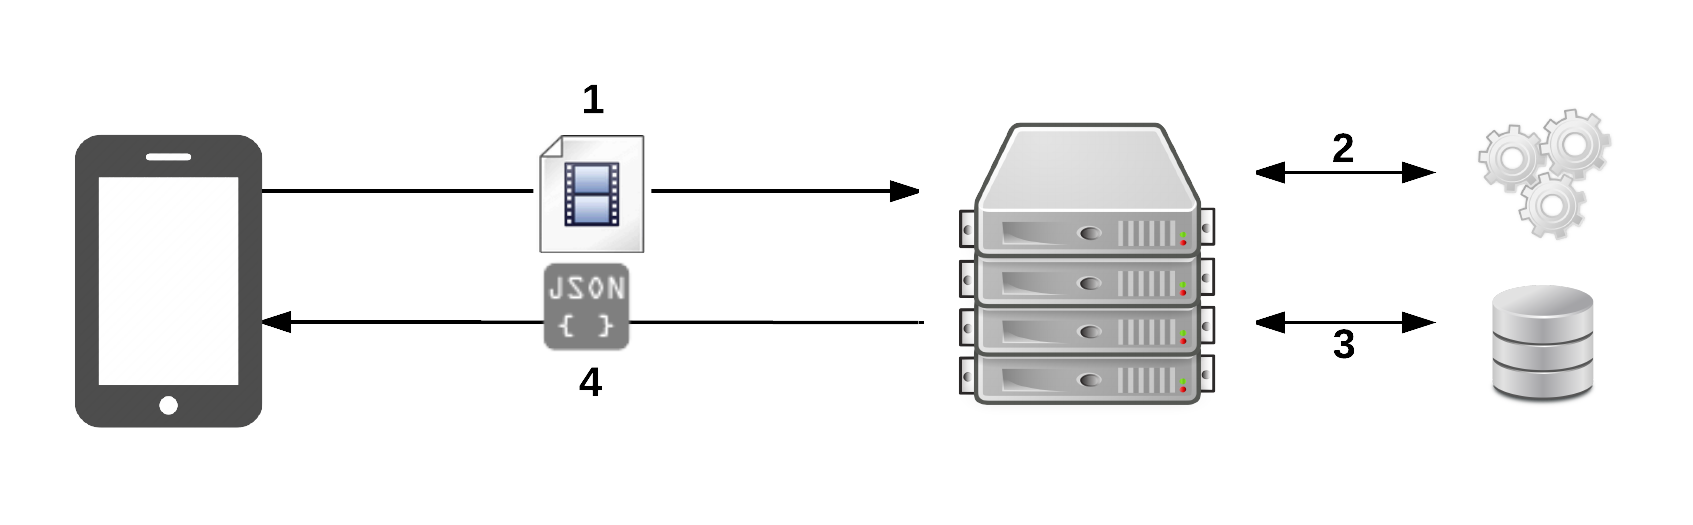
\includegraphics[scale=1]{imagenes/cap4/arquitectura_centralizada}
		\caption{Diagrama de la arquitectura del sistema centralizado.}
		\label{arquitectura_centralizada}
	\end{figure}
\subsection{Cliente Android}
En esta versión el cliente Android es responsable de grabar un video usando la cámara del dispositivo, enviarlo al servidor y de mostrarle al usuario los resultados de la búsqueda realizada por el servidor. Para cada una de estas responsabilidades se implementó un módulo.

\subsubsection*{Grabación}

El módulo de grabación es responsable de grabar un video usando la cámara del dispositivo y guardar el archivo resultante. Para lograr esto se creó el fragmento \texttt{VideoRecordFragment}, esta clase presenta al usuario un breve mensaje de instrucciones y un botón para comenzar la grabación. La figura ~\ref{pantalla_video_record_fragment} corresponde a la pantalla que ve el usuario al iniciar la aplicación. Al hacer click en el botón \emph{grabar} el sistema invoca a la aplicación por defecto de grabación de videos de Android por medio de un Intent.
La aplicación de grabación presenta un preview de la cámara como muestra la figura~\ref{pantalla_video_record_android}, en este momento el usuario debe iniciar la grabación, que dura por un máximo de 5 segundos y guarda en un archivo el video resultante. Después de terminar la grabación el sistema le cede de vuelta el control a la aplicación llamando al método \texttt{onActivityResult}, con esto se procede a enviar el video resultante al servidor.
\TODO{insertar aquí pantallazos de la aplicación}

\subsubsection*{Conexión con el servidor}
El módulo de conexión con el servidor es responsable de enviar al servidor el video capturado por el módulo anterior. Se implementó la clase \texttt{FromVideoSearchRequest} que recibe un archivo y ejecuta un petición HTTP Post al servidor usando la clase \texttt{HttpUrlConnection} de Java. Con la petición Post se envía el archivo grabado y un parámetro con el tipo de descriptor para usar en la búsqueda. Al crear un objeto de la clase \texttt{FromVideoSearchRequest} se le debe entregar un \texttt{ResponseHandler}, que corresponde a una interfaz con los métodos \texttt{onSuccessResponse} y \texttt{onFailure}, alguno de estos métodos se llamará dependiendo de la respuesta del servidor.
Una vez se termina el envío de datos al servidor se cambia la interfaz por una pantalla inicialmente vacía donde se mostraran los resultados como muestra la figura~\ref{pantalla_empty_results}.

\subsubsection*{Interfaz de resultados}
Para mostrarle los resultados de la búsqueda al usuario se implementó el fragmento \texttt{QueryResultsFragment} que implementa la interfaz \texttt{ResponseHandler} definida en la parte anterior. Inicialmente el fragmento muestra un texto indicando que se están esperando los resultados de la búsqueda, cuando se obtiene respuesta del servidor se ejecuta alguno de los métodos de la interfaz. Si el servidor responde con un error se ejecuta el método \texttt{onFailure} que muestra un mensaje al usuario informándolo del error. De lo contrario se ejecuta el método \texttt{onSuccessResponse} que recibe un String con los resultados del servidor codificados como JSON. Los resultados son deserializados usando la biblioteca GSON\footnote{GSON, biblioteca para convertir objetos Java a sus representación en JSON y vice-versa: \url{https://github.com/google/gson}} de manera que cada candidato de video identificado se convierte en un objeto de la clase \texttt{Detection} y se ingresa en una lista. El fragmento contiene un \texttt{ListView}, un elemento de interfaz de Android para mostrar listas de objetos. Se programó la clase \texttt{QueryResultAdapter} que recibe la lista de detecciones y crea una vista con cada una como muestra la figura~\ref{pantalla_list_results}.

El diagrama de la figura~\ref{diagrama_clases_centralizado} muestra las clases descritas en la sección anterior, detallando sus contenidos e interacciones.
	\begin{figure}[!h]
		\centering
		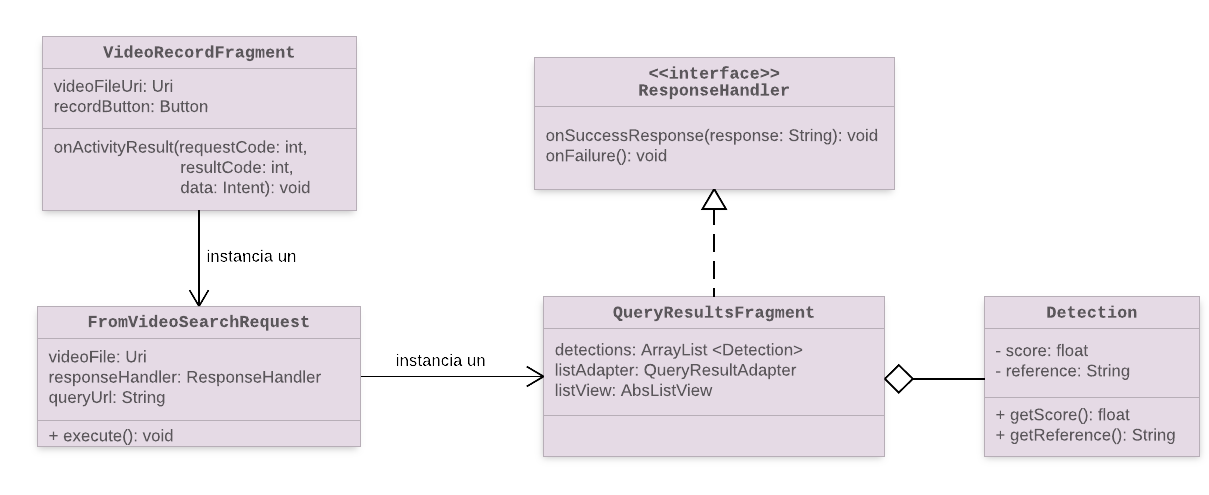
\includegraphics[scale=1.6]{imagenes/cap4/diagrama_cliente_centralizado.png}
		\caption{Diagrama de la arquitectura del sistema distribuido.}
		\label{diagrama_clases_centralizado}
	\end{figure}

\subsection{Servidor}

El servidor debe recibir una petición Post que contenga un video y el tipo de descriptor que se desea usar en la búsqueda. Debe usar el programa P-VCD para calcular los descriptores especificados y realizar la búsqueda para identificar el video original, finalmente debe entregarle al cliente en formato JSON una lista de los candidatos que encuentre.

Para recibir peticiones Post se usó el framework Flask, que permite programar servicios web con muy poco código extra. El siguiente ejemplo muestra todo el código necesario para definir y responder una petición Post:
\begin{lstlisting}[language=python]
from flask import Flask
app = Flask(__name__)

@app.route("/api/example/post", method=['POST'])
def hello():
	return "Hello World!"
	
if __name__ == "__main__":
	app.run(host='0.0.0.0')
\end{lstlisting}

La primera línea importa el módulo Flask, luego se define el objeto \texttt{app} que representa el contexto global de la aplicación. Para definir una request define una función con la anotación \texttt{@app.route}, explicitando la ruta y el tipo de petición. La función sirve una petición a la ruta especificada, dentro de la función se puede utilizar el objeto \texttt{app} para obtener el contenido de la petición. El string retornado por la función se convierte automáticamente en la respuesta del servidor.

Para servir la petición Post requerida se creó la función \texttt{search\_by\_video\_file} que escucha la URL host/api/search/search\_by\_video\_file.

\subsubsection*{Comunicación con P-VCD}
Como se detalló en capítulos anteriores P-VCD consta de múltiples módulos, cada uno con sus propio ejecutable que puede ser llamado por línea de comandos. Para usarlo en conjunto con el servidor para realizar el cálculo de descriptores y la búsqueda fue necesario encontrar la manera de ejecutar un programa externo desde Python.
Se encontró el módulo \texttt{subprocess}\footnote{Documentación del módulo subprocess: \url{https://docs.python.org/2/library/subprocess.html}} de Python que permite lanzar nuevos procesos pesados desde python de manera síncrona o asíncrona y obtener sus resultados. En particular se utilizó la función \texttt{call} de este módulo, que recibe una lista de strings con el nombre del programa y sus argumentos, lanza un nuevo proceso y espera a que termine, retornando el código de retorno del proceso.

Usando lo anterior se creó el módulo \texttt{PVCD\_Wrapper} que envuelve llamadas a las distintas etapas del proceso de búsqueda de P-VCD en funciones de python, a continuación se decriben las funciones usadas.
\begin{itemize}
\item \textbf{compute\_descriptors}: \\
La función recibe un archivo de video, un string correspondiente al tipo de descriptor a utilizar y un alias para el descriptor. Con esto realiza las llamadas necesarias para la extracción de descriptores de P-VCD, esto es, se llama a \texttt{pvcd\_db -new} para crear una nueva base de datos con el video correspondiente, luego se llama a \texttt{pvcd\_db -segment} para calcular su segmentación y finalemente se llama a \texttt{pvcd\_db -extract} para extraer el descriptor especificado.
\item \textbf{new\_search\_profile}: \\
Esta función recibe dos strings, uno con el nombre de la base de datos con los descriptores de consulta, y otro con el alias del descriptor y  realiza la llamada a \texttt{pvcd\_search -new} para crear un nuevo perfil de búsqueda.
\item \textbf{search}: \\
Esta función no recibe argumentos, llama a \texttt{pvcd\_search -ss} que toma los descriptores del video de consulta y para cada uno busca sus vecinos más cercanos en la base de datos de referencia.
\item \textbf{detect}: \\
Esta función no recibe argumentos llama a \texttt{pvcd\_detect} que usa la información de vecinos más cercanos del paso anterior para detectar secuencias al mismo video. P-VCD escribe en un archivo detections.txt la información de los videos que se consideran candidatos a ser el video original. La función lee este archivo y retorna una lista con el nombre de cada video y el puntaje de confianza que le asigna el sistema.

\end{itemize}
Usando estas funciones el código de la función \texttt{search\_by\_video\_file} queda como sigue:
\begin{lstlisting}[language=python]
@app.route("/search/api/search_by_video_file", methods=['POST'])
def search_by_video_file():
  if request.method == 'POST':
    uploaded_file = request.files['uploaded_file']
    if uploaded_file and allowed_file(uploaded_file.filename):
      db_name = 'query'
      descriptor = request.form['descriptor']
      alias = request.form['alias']
      file_path = save_video_file(uploaded_file)
      PVCD_Wrapper.compute_descriptors(file_path, descriptor, alias)
      PVCD_Wrapper.new_search_profile(db_name, alias)
      PVCD_Wrapper.search()
      detections = PVCD_Wrapper.detect()
      
      return jsonify(detections=detections)
\end{lstlisting}
Primero se verifica que la petición sea de tipo Post y que se haya recibido un video con formato válido. Luego la función ejecuta secuencialmente los pasos de la búsqueda y retorna los resultados usando la función \texttt{jsonify} de Flask, que codifica una lista de Python como JSON.


\section{Sistema Distribuido}

La figura~\ref{arquitectura_distribuida} ilustra la arquitectura de esta versión del sistema. El cálculo de descriptores para la búsqueda es realizado por el cliente Android (1) utilizando las herramientas para computación paralela descritas en secciones anteriores. Una vez calculados, se envían solo estos descriptores al servidor (2) el cual los usa para realizar la búsqueda por similitud (3) y luego comunica los resultados de vuelta al cliente (4).

	\begin{figure}[!h]
		\centering
		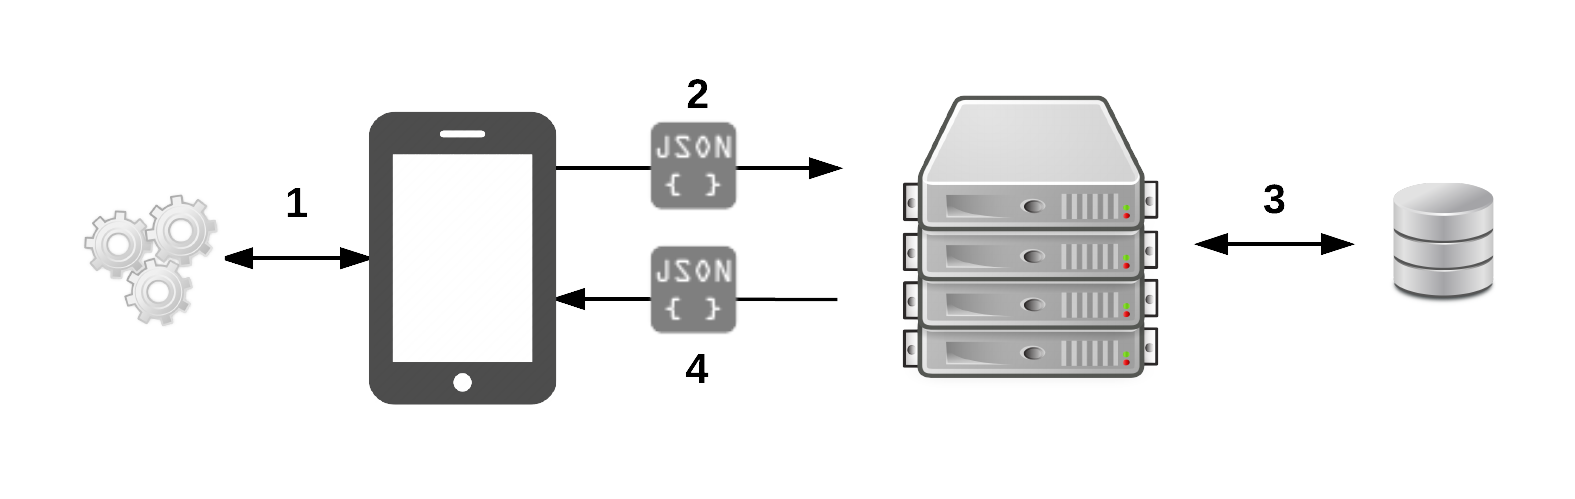
\includegraphics[scale=1]{imagenes/cap4/arquitectura_distribuida.png}
		\caption{Diagrama de la arquitectura del sistema distribuido.}
		\label{arquitectura_distribuida}
	\end{figure}

A continuación se detalla la implementación de tanto el cliente Android como el servidor y se comentan las diferencias con respecto a la versión descrita anteriormente.

\subsection{Cliente Android}
A diferencia de la versión anterior del sistema, en esta versión el cliente debe calcular los descriptores del video de consulta y realizar un petición Post al servidor enviando solo los descriptores y no el archivo de video completo. Al igual que la versión centralizada una vez obtenida la respuesta del servidor, debe mostrarle los resultados de la búsqueda al usuario. Se implementó esta versión cambiando el módulo de grabación de la cámara y el de conexión con el servidor, además se añadió un módulo de cálculo de descriptores.

\subsubsection*{Grabación}
En esta versión ya no es necesario obtener un archivo de video resultante, sino que es necesario realizar un procesamiento del video. Dada esta diferencia se decidió reimplementar este módulo, creando un nuevo fragmento \texttt{CameraPreviewFragment} de manera que se puedan obtener frames de la cámara mientras se graba el video, para poder realizar el cálculo en tiempo real.

La interfaz gráfica del fragmento \texttt{CameraPreviewFragment} consta de tres elementos que podemos identificar en la figura~\ref{pantalla_camera_preview}, el preview de la cámara, los cuatro puntos con los que el usuario puede marcar los límites de la pantalla y finalmente un botón para comenzar la grabación. A continuación se detallan aspectos de la implementación de cada uno de estos elementos.

A diferencia de la versión anterior, en que la cámara era manejada por una aplicación predefinida, ahora es necesario manejar los eventos del ciclo de vida de la cámara. Para esto se utilizó la funcionalidad de la clase \texttt{Camera}\footnote{\url{http://developer.android.com/guide/topics/media/camera.html}} de Android. Esta clase permite mostrar un preview y obtener frames para procesarlos en tiempo real. Se programó la clase \texttt{CameraContainer}, que representa un elemento gráfico que contiene el preview. La clase además encapsula las llamadas al sistema operativo necesarias para controlar la cámara, a través de las funciones \texttt{startCameraPreview}, \texttt{stopCameraPreview} y \texttt{releaseCamera}. 

Se programó la clase \texttt{CropView} que controla los cuatro puntos ...







\subsection{Servidor}
